\chapter{Background}
\label{chp:background} 

This thesis describes the setup and usage of an End-to-End \gls{iot} system. In order for this to be set up by others later to perform reproducible tests, a detailed description of components, sensors and protocols used is needed. This chapter will go through the background information of the devices, technologies and protocols used, and why these where chosen over other alternatives. 

%\section{Internet of Things} % Tjae

%Comment: Read Future Internet: The Internet of Things from 2010.  \cite{gubbi2013internet}

%Comment: Read http://ac.els-cdn.com/S1570870512000674/1-s2.0-S1570870512000674-main.pdf?_tid=6f15526e-eae8-11e5-addc-00000aab0f6b&acdnat=1458072152_0740a71f559cd8ae1ebd0ce4a687e122

%M2M and "M2T" ("Machine to Thing-communication"). Classification of a thing? \cite{tan2010future}. 

%\section{Challenges}

\section{Hardware}

The hardware section will go through the physical devices used to build the \gls{iot} network, which is central to solve objective O.1. 

\subsection{Raspberry Pi}

Developed by Newark Element 14, the Raspberry Pi has become a central tool for many people wanting to get started using small computers \cite{newark}. The device has been known as a single-board computer the size of a credit card specially designed for small network projects and to be used as an educational tool used all the way from elementary schools to here at \gls{ntnu}. This was therefore a natural device to use as a starting point in this system as well. 

\begin{figure}[ht]
    \centering
    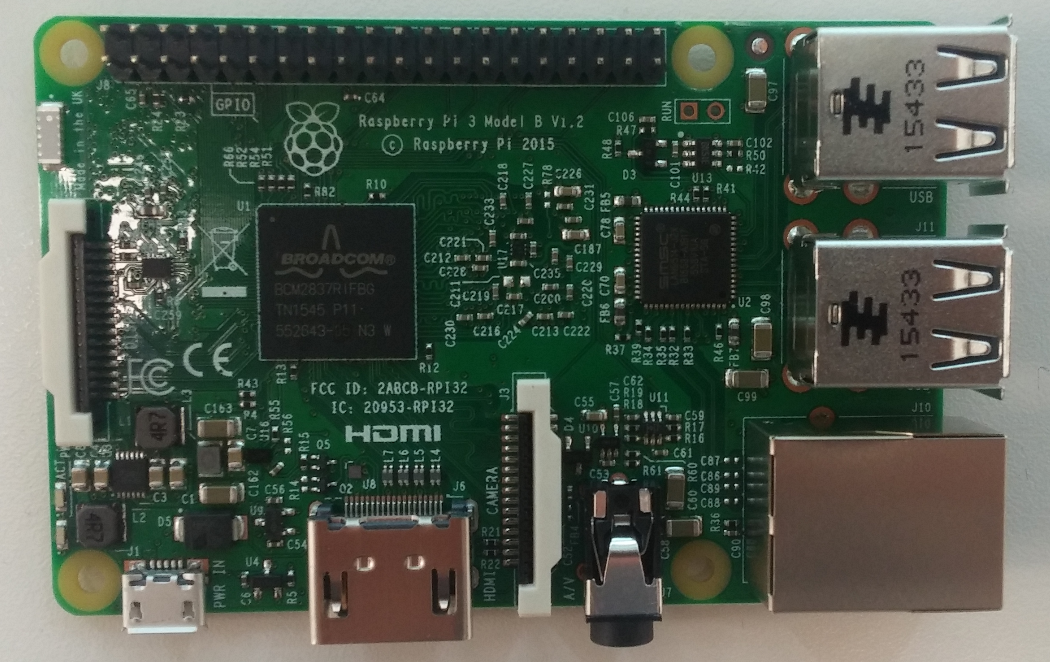
\includegraphics[scale=0.35]{pi3.png}    
    \caption{Raspberry Pi 3}
    \label{fig:piPicture}
\end{figure}

The Raspberry Pi is a \gls{singleBoardComputer} on the size of a credit card. Model 3 of this was released in February 2016, just in time to become a part of the system set up in this project. This includes a \gls{cpu} speed of 1,2 GHz and 1 GB of \gls{ram}. This makes it approximately 12 times faster than the first Raspberry Pi. Both Bluetooth and WiFi is included, and it was quite easy to set up, given that the right Unix kernel has been used in the \gls{os} of the Pi. Along with the Raspberry Pi, we needed a good and stable operating system with a kernel that supported the \gls{6lowpan} architecture. For this, Ubuntu Mate version 15.10 with kernel version 4.15 was chosen, and used on the Raspberry Pi. As other versions of Ubuntu this is Unix based, and has a complete \gls{gui} of a full \gls{os}. The set up of this will be explained in chapter \ref{chp:architecture}.1. 

\subsection{nRF52}

The most central device of this network is the microcontroller used as end-nodes, the nRF52 developed by Nordic Semiconductor with the \gls{iot} development kit. This is presented as a family of highly flexible, multi-protocol system on chip devices. 


\begin{figure}[ht]
    \centering
    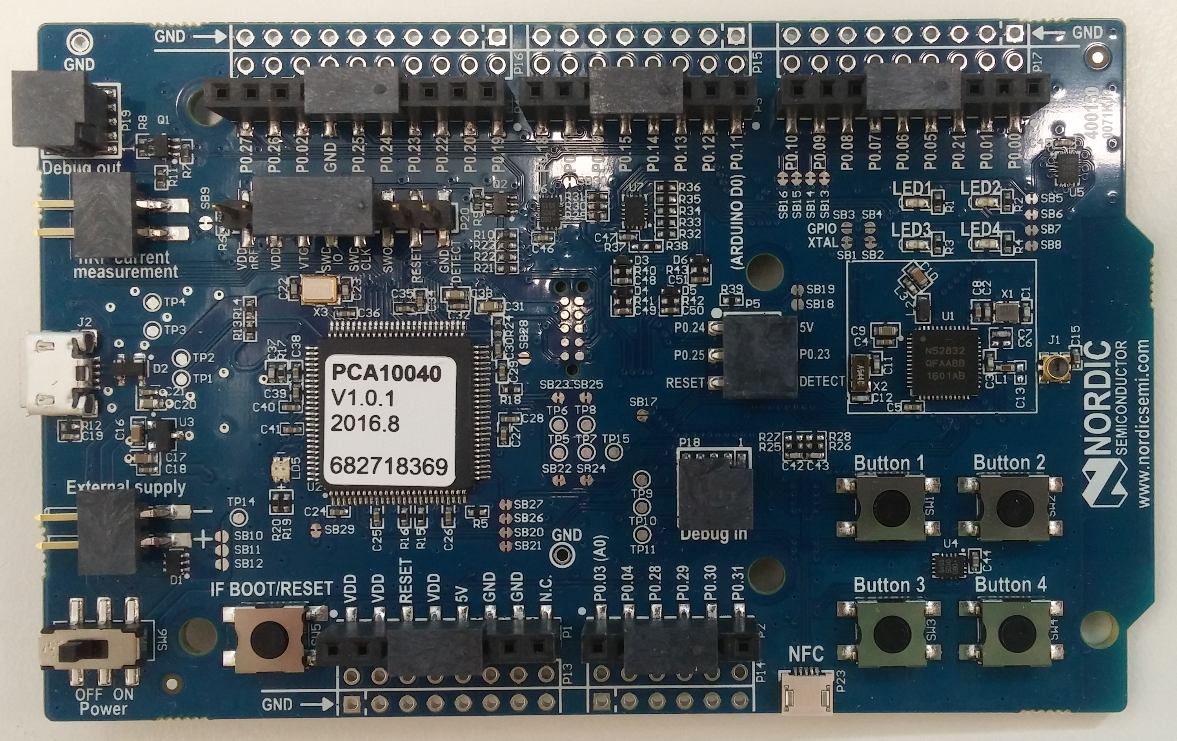
\includegraphics[width=1.0\textwidth]{nRF522.png}    
    \caption{Nordic Semiconductor nRF52 }
    \label{fig:nrf52picture}
\end{figure}


This device has been advertised as a powerful multiprotocol single chip solution, with both a 32-bit ARM processor, a 512kB flash and 64kB og flash memory. The building blocks of the chip in its entirety is shown in \ref{fig:nrf52chipDetail}. The key features mentioned by Nordic Semiconductor \cite{nrf52Nordic} that will be relevant in this network are: 

\begin{itemize}
	\item Multi-protocol 2.4GHz radio
	\item 32-bit ARM Cortex M4F processor
	\item 512kB flash + 64kB RAM
	\item Application development independent from protocol stack
	\item Dynamic on air payload length up to 256 Bytes
	\item Flexible and configurable 32 pin GPIO
	\item Programmable Peripheral Interface – PPI
	\item Full set of digital interfaces including: SPI/2-wire/UART/PDM/
	\item I2S, all with EasyDMA
	\item Low cost external crystal 32MHz ± 40ppm for Bluetooth, ± 50ppm for ANT
	\item Wide supply voltage range (1.7 V to 3.6 V)
	\item On-chip DC/DC buck converter
\end{itemize}


The most interesting points here are the processing power, the flash storage and \gls{ram}, the \gls{i2c} and \gls{spi} buses and the bluetooth antenna. 

%\cite{nrf52Nordic2}


\begin{figure}[ht]
    \centering
    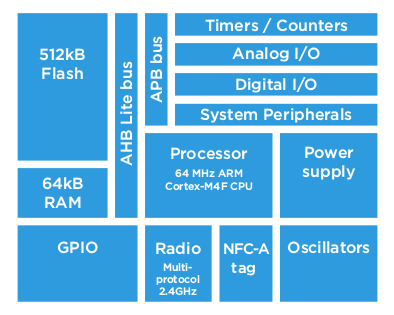
\includegraphics[scale=0.6]{nrf52Detailed.png}    
    \caption{Nordic Semiconductor nRF52 chip in detail }
    \label{fig:nrf52chipDetail}
\end{figure} 

Figure \ref{fig:nrf52chipDetail} shows how the different sections are distributed on the nRF52832 \gls{soc} \ref{fig:nrf52chipDetail}.  

% https://www.nordicsemi.com/Products/nRF52-Series-SoC
A SoftDevice is a precompiled binary software that implements \gls{ble} on the nRF52. This means that the user can start to work directly in a standard C language interface, which is independent from the Soft Device implementation \cite{softDevice}. This makes it possible for users to write strandard programming code instead of require a deep knowledge of device specific configurations. There are several versions of SoftDevices to the nRF52 that can be downloaded from \url{http://www.nordicsemi.com}. 


\subsection{Adafruit ADXL345 Accelerometer}

As seen in the previous section, the nRF52 has good computational power for a \gls{microcontroller}, and several possibilities when it comes to radio communication. But in addition to this, an external sensor was needed to collect data. Supporting both the \gls{i2c} and \gls{spi}, the nRF52 has got the most standard interfaces needed to do this build in. Objectives presented in the introduction to this thesis states that is preferable both to collect, transport and analyse data in this network. The sensor chosen to do this was the ADXL345 accelerometer from Adafriut. This was selected for the following main reasons:  

\begin{itemize}
  \item It can measure acceleration in all three axes, X, Y and Z.
  \item It sends digital data right away. This means there is no need to use computational power to calculate digital values as needed if the data was captured by an analog accelerometer. 
  \item It supports both \gls{i2c} and \gls{spi}, which makes it easy to connect to the nRF52. 
  \item It supports voltage of 3.3V-5.0V, which fits within the range of output from the nRF52.  
\end{itemize}


%\begin{figure}[ht]
%    \centering
%    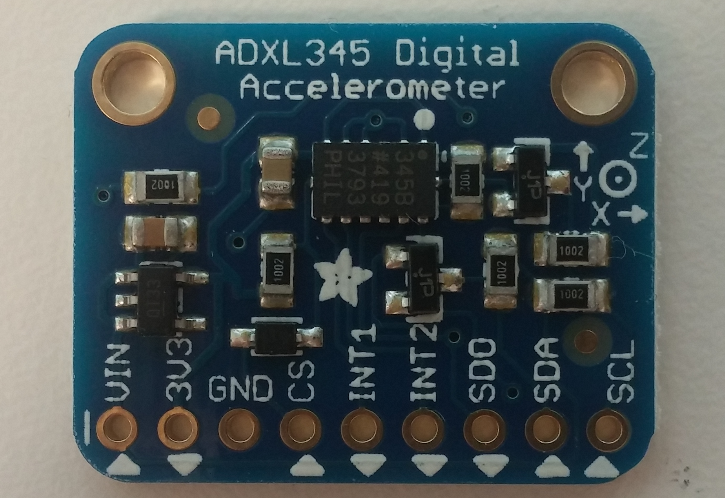
\includegraphics[scale=0.32]{ADXL345.png}    
%    \caption{ADXL345 Accelerometer}
%    \label{fig:adxl345}
%\end{figure}


\begin{figure}[ht]
    \centering
    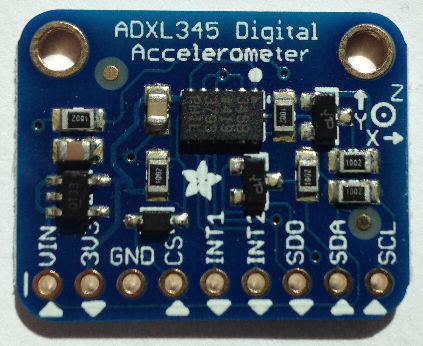
\includegraphics[width=0.5\textwidth]{adxl345imagge}    
    \caption{ADXL345 Accelerometer}
    \label{fig:adxl345}
\end{figure}

When connecting to the \gls{nRF52}, using the \gls{i2c} interface was chosen because it is simple with few cables, supports an acceptable bit rate and several sensors in the same link. Ports VIN, GND, SDA and SCL will be used in this connection, which will be explained in detail in chapter \ref{chp:architecture}. 

\subsection{Additional computational power}

Devices presented so far are small network devices with limited or no computational power, that can be used as end nodes or more central nodes in an \gls{iot} network. The Raspberry Pi already has network connectivity, and can therefore be used as the final node before the results are presented on a screen, a web page or to be stored on a server. In many cases however, it will be an advantage to include another node with a lot more computational power before the results are being published. This both limits the computations needed to be done at the Raspberry Pi, and means that the system are able to do more deep analyses of the data gathered from the system, without the fear of a system overload. A central stationary computer, a supercomputer or computational power from a web service are possible solutions. In this network a standard stationary computer running a Linux Ubuntu based system was used as this node. Because of the limited time provided for this thesis the scope focuses mostly on data analysing and transportation between small nodes in an end-to-end \gls{iot} system. The results were mostly obtained and calculated on the Raspberry Pi, meaning this last central node was not much used in this solution. This could however be a central topic for future projects aiming to more complex data analysis. 

\subsection{Alternative devices}

There was never considered an alternative for the Raspberry Pi, since this is a well known device with a good reputation. This should mean that it would be easy to use, easy to find advices and help when needed, and easy get hold on devices when needed. There are of course other alternatives available, for instance the Ardurino Uno, Banana Pi or the BeagleBone Black, that could have been considered if there where any problems with the Raspberry Pi. The main contestant to replace the nRF52 was the Zolertia Z1 microcontroller. This was a good alternative to use since it already has got an accelerometer fitted on the board. It does not have the same computational power as the nRF52, and Nordic Semiconductor is a well known company based in Trondheim. This therefore seemed like a very interesting device to be tested in a thesis at \gls{ntnu}. Should there have been any problems with the nRF52 the Zolertia Z1 would have been a natural contestant as a replacement. ADXL345 is the same accelerometer built in on the Zolertia Z1 microcontroller. This was therefore a natural choise when these two microcontroller where considered the main candidates in the network. If future works will do similar tests later, the results will be comparable between these two. 


\section{Communication technologies}

After the devices to use had been selected, the next step was to find relevant communication technologies that could be used to establish a reliable, fast and low power connection between the \gls{nRF52} and the \gls{Raspberry Pi}. 

\subsection{Bluetooth Low Energy}

\gls{ble}, also known as \textit{Bluetooth Smart}, is a wireless technology for short range communication developed by the Bluetooth Special Interest Group. The idea was to create a low energy single-hop network solution for \glspl{pan}. A major advantage of this solution is that Bluetooth 4.0 already is a well established technology in cell phones, laptops and several other devices. This means that few changes needs to be made to these devices to be able to work with bluetooth smart. Still to this date, a device that only implements \gls{ble} is not able to communicate with a device that only implements classic Bluetooth \cite{gomez2012overview}.
The 6LoWPAN Working Group has recognized the importance if \gls{ble} in \gls{iot} \cite{hui2008extending} \todo{Denne linken snakker om 6lowpan, flytte til etter jeg har presentert 6LoWPAN?}.

\begin{figure}[ht]
    \centering
    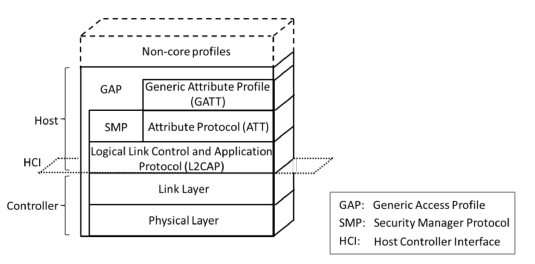
\includegraphics[scale=0.7]{BLEprotocolStack.png}    
    \caption{BLE protocol stack}
    \label{fig:BLEprotocolStack}
\end{figure}

The protocol stack of \gls{ble} has two main parts, the controller and the host, as shown in \ref{fig:BLEprotocolStack} \cite{gomez2012overview}. In the system presented in this thesis this represents the Raspberry Pi as the controller (master) and Nordic nRF52 as the host (slave). The communication between these is done through the standard \gls{hci}, a bluetooth protocol. All slaves are in sleep mode by default, and are woken up by the master when communication is needed. Links are being identified by a randomly generated 32-bit code, and the \gls{ism} band used is 2,4 GHz \cite{gomez2012overview}. Other protocols used include \gls{l2cap} used to multiplex data between higher protocol layers, and the segmentation and reassembly of packets. From here packets are being passed to the \gls{hci}, which is the interface used to communicate between the two \gls{ble} devices. This is being used in conjunction with \gls{acl}, which is used to create the \gls{tdma} scheme used to transfer packets over the network link, as well as controlling uptime of the end nodes, as this link is set to disconnect automatically after a given time period if there is no activity on the link. Concrete examples of these protocols will be shown later in the thesis. 



\begin{figure}[ht]
    \centering
    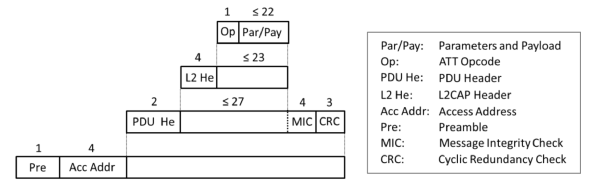
\includegraphics[scale=0.7]{BLEdataUnitStructure.png}    
    \caption{BLE Data Unit Structure}
    \label{fig:BLEdataUnitStructure}
\end{figure}

Figure \ref{fig:BLEdataUnitStructure} shows the data unit structure in \gls{ble}, meaning the different fields that can be used in a packet \cite{gomez2012overview}. The header fields of 4 \gls{byte} of access addresses and \gls{l2cap} will be central topics of discussion later in this thesis. In the case of the network presented here, when the \gls{ble} slave has been connected to a master, it stops searching for other connectible points. This means that it is not possible to connect to several masters, and it will only be possible create a \textit{star network}, not a \textit{mesh network}. A mesh network would in many cases be preferable, since \gls{ble} is considered a \gls{pan} with a very limited range. In a mesh network end nodes can communicate with each other, meaning they can span a larger area without the need of a central and common point of connection. This could possibly be an idea for improvement later. Other than this, \gls{ble} seems like a very good alternative in this project. 

%Check out: Mikhail Galeev - BLE

\subsection{6LoWPAN}

%To identify sensors and devices in low energy sensor and device networks, a new protocol was needed. 

\gls{6lowpan} is a defined protocol for using \gls{ipv6} in low energy networks, to identify sensors and devices, as defined in the IEEE 802.15.4. To use the Internet Protocol in low energy networks in addition to standard networks was proposed by Geoff Mulligan and the 6LoWPAN Working Group. This was chosen because it seemed like a simple and smart protocol definition. Since packets in this network can end up being forwarded all the way from a \ref{microcontroller} to a central computer through several nodes without being changed, it makes sense to use the same base protocol for all links. In \cite{mulligan20076lowpan}, the advantage of \gls{6lowpan} is explained as 

\noindent\textit{Utilizing IP  in these networks and pushing it to the very edge of the network devices flattens the naming and addressing hierarchy and  thereby  simplifies  the  connectivity  model. This obviates the need  for  complex  gateways  that,  in  the  past,  were  necessary  to translate   between   proprietary   protocols   and   standard   Internet Protocols and instead can be replaced with much simpler bridges and  routers,  both  of  which  are  well  understood, well  developed and  widely  available  technologies \cite{mulligan20076lowpan}.}


\gls{6lowpan} was developed to be used in small sensor networks, and implementations can fit into 32Kb flash memory parts. The \gls{mtu} is given to be 1280 byte, and it also uses a complex header comparison mechanism that allows the transmission of \gls{ipv6} packets in 4 bytes, much less than the standard \gls{ipv6} 40 bytes. This is done by using stacked headers, same as in the \gls{ipv6} model, rather than defining a specific header as for \gls{ipv4}. The device can send only the required part of the stack header, and does not need to include header fields for networking and fragmentation \cite{hui2008extending}. The maximum packet size of the physical layer is set to be 127 bytes, far below the limit of 1280 byte \cite{kushalnagar2007transmission}. It is expected that other layers will produce packets of the desired size to fit the system. In the system presented in this thesis by the example code on the nRF52 is the side set to 270 bytes for every packet, as will be shown in practical examples and tests later in the thesis. 


%The \gls{6lowpan} architecture was developed to allow \gls{ipv6} packets to be sent over low energy networks.  

\subsection{Other alternatives}

\textit{ANT} was the main other alternative to \gls{ble} when network protocols where chosen. It also uses  the 2,4 GHz ISM band, and is made to be used in sensor based networks \cite{ant}. It is supported by the \gls{nRF52}, and could be used with a \gls{Raspberry Pi} if an ANT \gls{usb} dongle is fitted. This would have solved the \gls{ble} problem with not being able to connect several devices together in a mesh network, since ANT supports this. Other than this the difference is not very large. \gls{ble} is supported by other mobile devices on the other hand, meaning it is possible to use a mobile application developed by Nordic Semiconductor to test the connection. This was assumed to be a very useful feature, and was one of the main reasons why \gls{ble} was chosen. 

Two other contestants than \gls{6lowpan} was \textit{Zigbee} and \textit{Zensys}, being compared directly in \cite{mulligan20076lowpan}. The major factors here are that \gls{6lowpan} has a much higher network size than the others, supports Internet connectivity using routers as well as the use of \gls{udp} and \gls{tcp}, supports low amounts of \gls{ram} and small headers \cite{mulligan20076lowpan}. 


\section{Transport protocols}

In order to transfer data from the end nodes to the central points of the network, either for analysing or already analysed data, a fast, efficient and stable transport protocol has to be used. This is a central aspect in this network, because the limitations of sending rate is thought to be one of the main limitations, either in the form of limits of data at once or number of transmissions per second. The protocol needs to be stable and energy efficient and work with both \gls{ble} and \gls{6lowpan}. Luckily, Nordic Semiconductor provides example code and examples on how to get started with this.

\subsection{CoAP}

%The \\ protocol is described in the documentation as follows: 

\gls{coap} is a transport protocol designed to be used in constrained networks for \gls{m2m} communication. It is \gls{udp} based, and works good in low-power and lossy networks. It can be used with microcontrollers, and with \gls{ipv6} and \gls{6lowpan}. Both GET and PUSH functionality can be used, as well as \textit{observable} GET. This means that a server can "subscribe" to end notes in the network, and get updates either after a given timespan or when changes have been made. This therefore looked like a promising protocol to use, and was chosen as the main transport protocol to test in the network \cite{shelby2014constrained}. The main technical features described in \gls{coap} includes fulfilling \gls{m2m} requirements, support of asynchronous messages, gls{udp} based communication and stateless mapping to \gls{http}. 

CoAP has several similarities with \gls{http}, using the same client and server roles. The client sends a request, and the server sends a response back. Many of the response codes are also very similar, with \textit{404: Not found} as the best known. When \gls{m2m} communication is used, both participants sometimes needs to be both client and server, and the \gls {coap} protocol handles this with a two-layer approach. \todo{make figure of CoAP Layering}. There are four different main messages defined in gls{coap} \cite{shelby2014constrained}. 

\begin{itemize}
	\item A Confirmable message, \gls{con}, require one \gls{ack} for every packet received. If a message is not received correctly, the receiver will ask for exactly return message of the type Acknowledgement. 
	\item A Non-confirmable message, \gls{non}, does not require an \gls{ack}. This means a higher possibility of a packet getting lost, especially in lossy networks, but it requires less capacity from the network and should in general be faster. 
	\item An Acknowledgement acknowledges that a specific \gls{con} packet has reached its destination. 
	\item A Reset message tells the sender that a specific message was received, but some content is missing to be able to understand it, for instance if the receiver has had a reboot during the transmission. An empty Reset message represents a ping test of \gls{rtt}, which will be used when testing a connection. 
\end{itemize}
      
Other commands used in \gls{coap} are \textit{GET, PUT, POST and DELETE}, to get or change data. 

%Figure \ref{fig:layersCoAP} 
%\begin{figure}[ht]
%    \centering
%    \includegraphics[scale=0.5]{seqDiagramCoAP.png}    
%    \caption{Layers in CoAP}
%    \label{fig:layersCoAP}
%\end{figure}


\begin{figure}[ht]
    \centering
    \includegraphics[scale=0.6]{CONclientserver.png}    
    \caption{CON CoAP set up sequence diagram}
    \label{fig:CONclientserver}
\end{figure}

Figure \ref{fig:NONOackSeqDiagram} shows the basic message sequence between the client and the server in a \gls{coap} \gls{con} network. Every request CON message needs to be given an ack back. 

\begin{figure}[ht]
    \centering
    \includegraphics[scale=0.6]{NONOackSeqDiagram.png}    
    \caption{NON CoAP set up sequence diagram}
    \label{fig:NONOackSeqDiagram}
\end{figure}

Figure \ref{fig:CoAPMessageFormat} shows the same for \gls{non}, where no \glspl{ack} are needed. The same initial set up with con and ack messages are still needed, to establish a connection between the client and server before a stream of \gls{non} messages can be sent. This means a much more unreliable connection than using \gls{con}, since messages can be dropped without either the client or the server gets notified. Systems where a few packets can be lost without difficulties, for instance in a sensor based network like the network presented in this thesis, can use this as an advantage. A message ID is still provided to every message to remove duplicated messages, but dropped messages are lost data. If the packages sent contained data that could not be dropped, for instance containing crucial patient information from censors on a patients body, this is not a good solution. The more reliable solution \gls{con} is a much better alternative in this case. These differences are the same as being experienced in the \gls{iot} system described in this thesis, which can be seen in figure \ref{fig:CoAPNONwiresharkSetUp}. A \gls{con} message is sent several times, to set up the initial connection. When an \gls{ack} is received as a response, the continuous transportation of \gls{non} packets without \glspl{ack} can begin. 

\begin{figure}[ht]
    \centering
    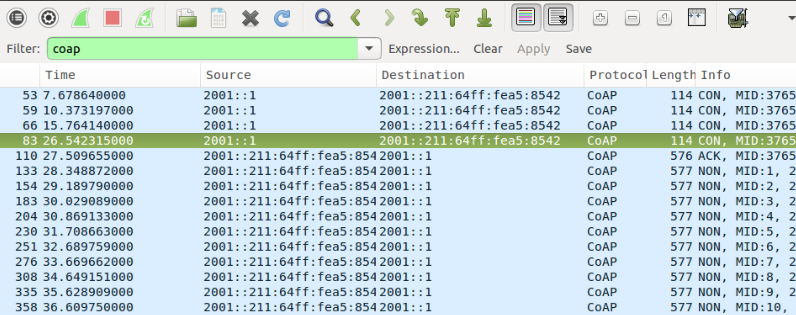
\includegraphics[width=1.0\textwidth]{coapCONwiresharksetUpSequence.png}    
    \caption{CoAP NON, set up sequence, Wireshark capture}
    \label{fig:CoAPNONwiresharkSetUp}
\end{figure}

%\todo{Show examples of setting up coap NON needs acks first? Wireshark without bluetooth-sniffing?}

The message format used in \gls{coap} is very simple, and can be seen in figure \ref{fig:CoAPMessageFormat}. The 4 first byte are header files, followed by optional tokens and options. When these are not being used, like in this network, the minimal header size of either 4 or 5 bytes. This is a huge advantage in \gls{iot} networks.


\begin{figure}[ht]
    \centering
    \includegraphics[scale=0.6]{CoAPMessageFormat.png}    
    \caption{CoAP message format}
    \label{fig:CoAPMessageFormat}
\end{figure}



%\begin{figure}[ht]
%    \centering
%    \includegraphics[scale=0.6]{CoAPUsageOfMessageTypes.png}    
%    \caption{CoAP usage of message types}
%    \label{fig:CoAPUsageOfMessageTypes}
%\end{figure}



\subsection{MQTT}

An alterntive transport protocol in a system such as this is \gls{mqtt}. This is  known as a publish-subscribe messaging system based on \gls{tcp} for \gls{m2m} communication. A client will in this case \textit{subscribe} to a \textit{publisher} in the network \cite{hunkeler2008mqtt}. When a publisher updates a field of interest for the subscriber, the subscriber will get notified. Subscriptions are being coordinated by a \textit{broker}, as seen in figure \ref{fig:mqttSeqDiagram}. Messages sent in such a network are either \textit{sub(topic)} to subscribe to a topic, or \textit{pub(topic, data)} to publish data \cite{mqttWebsite}. 


\begin{figure}[ht]
    \centering
    \includegraphics[width=0.8\textwidth]{mqttSeqDiagram.png}    
    \caption{MQTT subscription sequence diagram}
    \label{fig:mqttSeqDiagram}
\end{figure}

\gls{mqtt} supports end-to-end \gls{qos}, and has a simple and good message architecture. This protocol would also be possible to use in such a system. Because of the limited time frame of this thesis however, it was decided to study \gls{coap} in depth first, and leave the testing of \gls{mqtt} to future work. 



\section{Software tools}

As \gls{ide}, the \textit{KEIL Vision} was used, as recommended by Nordic Semiconductor in \cite{nordicSoftwareTools}, for writing C programming. For other programming languages (for instance Python 3.4)  Text 2 for Windows and Linux was used, as well as \textit{Pluma} for Ubuntu Mate on the Raspberry Pi. 

\subsection{Wireshark}

Wireshark is a software tool to analyse networks and capture packets sent using different technologies 

\subsection{Copper}

Copper is a generic browser which can be used in \textit{Firefox}. It is 
\cite{kovatsch2011demo}

\begin{figure}[ht]
    \centering
    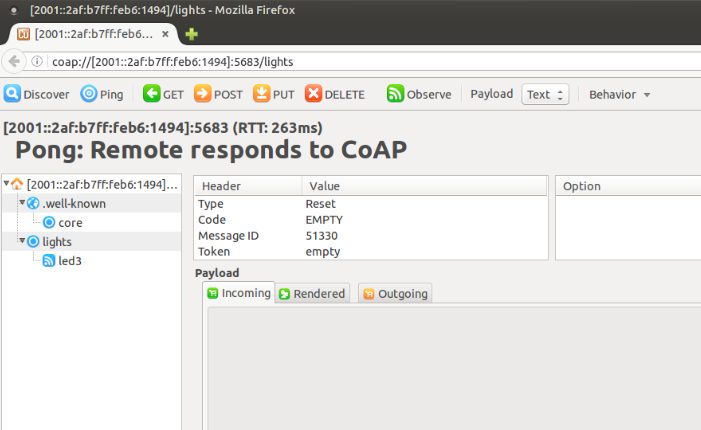
\includegraphics[width=1.0\textwidth]{CopperExample.png}    
    \caption{\textsc{Copper example}}
    \label{fig:copperExample}
\end{figure}

\gls{radvd} is a software tool that can be used to advertise \gls{ipv6} addresses in a local network, using \gls{ndp} \cite{chown2011rogue}. . This is being used to multicast and forward packets in this network. When a packet is sent from an end node to another, the communication needs to go through the central point in the star network, the Raspberry Pi in this case. Here, \gls{radvd} ensures that the packages are being routed to the right end point, or the right nRF52 in this system. 

Other software used to set up, monitor and test this network include Mozilla Firefox with Copper \todo{image?} to get basic communication with nRF52 from the Pi without the use of a script or terminal. Wireshark has been used to capture packets sent through the network, and GitHub has been used both as a backup solution. To make the most basic figures in this thesis the web based tool \textit{draw.io} was used, unless other is specified. \textit{polt.ly} was used to draw the graphs used. All the images of devices in the network has been taken by the author. 

\subsection{Other}
